\subsection{Main Results}
\label{sec:results}

\paragraph{Comparison across embodied benchmarks.}

\begin{table*}[!htbp]
\caption{Cross-benchmark comparison (\%; best values in bold).
For \evolvingworldnav{}, $\pm$ denotes the standard deviation over five seeds.}
\label{tab:crossbench}
\centering
\scriptsize
\setlength{\tabcolsep}{4.0pt}
\resizebox{\textwidth}{!}{%
\begin{tabular}{lcccccccc}
\toprule
& \multicolumn{2}{c}{\textbf{FindingDory}} &
\multicolumn{3}{c}{\textbf{GOAT-Bench}} &
\multicolumn{3}{c}{\textbf{\evolvingworldbench{}}}\\
\cmidrule(lr){2-3}\cmidrule(lr){4-6}\cmidrule(lr){7-9}
\textbf{Method} & \textbf{HL-SR $\uparrow$} & \textbf{HL-SPL $\uparrow$} &
\textbf{SR $\uparrow$} & \textbf{SPL $\uparrow$} &
\textbf{Repeat-SR $\uparrow$} & \textbf{First-Inspection SR $\uparrow$} &
\textbf{Search SR $\uparrow$} & \textbf{SPL $\uparrow$}\\
\midrule
\rowcolor{tblnav}\multicolumn{9}{c}{Open-vocabulary and lifelong navigation}\\
VLFM \citep{yokoyama2024vlfm} & 13.42 & 10.86 & 15.79 & 5.45 & 11.82 & 20.65 & 28.36 & 24.67\\
ZSON \citep{majumdar2022zson} & 27.89 & 21.81 & 29.64 & 2.45 & 16.37 & 26.84 & 32.13 & 28.55\\
FindingDory Agent \citep{yadav2025findingdory} & \paperreported{52.44} & \na & \na & \na & \na & \na & \na & \na\\
LagMemo GLUE \citep{zhou2025lagmemo} & 32.79 & 23.25 & 20.61 & 1.74 & 11.27 & 30.18 & 42.27 & 33.82\\
\midrule
\rowcolor{tblmemory}\multicolumn{9}{c}{Structured spatio-temporal memory}\\
HOV-SG \citep{werby2024hovsg} & 21.47 & 15.20 & 28.37 & 2.23 & 12.38 & 36.46 & 52.32 & 40.61\\
DynaMem \citep{liu2024dynamem} & 30.30 & 22.78 & 14.54 & 1.71 & 15.79 & 45.33 & 71.94 & 56.83\\
\midrule
\rowcolor{tblpredict}\multicolumn{9}{c}{Predictive world and state modeling}\\
SLaTe-PRO \citep{patel2023routine} & 18.18 & 14.53 & 9.41 & 0.99 & 6.38 & 13.00 & 36.33 & 26.37\\
SGM+NEP \citep{kurenkov2023dynamic} & 34.20 & 19.48 & 10.67 & 1.64 & 2.56 & 27.26 & 41.82 & 37.00\\
FlowMaps \citep{argenziano2026flowmaps} & 13.03 & 10.24 & 25.07 & 1.32 & 7.25 & 14.33 & 32.67 & 17.35\\
PredictiveGraphs \citep{saavedraruiz2026predictivegraphs} & 24.24 & 13.50 & 10.27 & 1.80 & 7.48 & 36.18 & 43.67 & 40.36\\
\midrule
\rowcolor{tblours} & \textbf{53.22} & \textbf{38.83} &
\textbf{35.43} & \textbf{12.98} & \textbf{19.31} & \textbf{61.32} &
\textbf{86.18} & \textbf{70.15}\\
\rowcolor{tblours}\multirow{-2}{*}{\textbf{\evolvingworldnav{} (ours)}} & $\pm 3.87$ & $\pm 2.43$ & $\pm 2.16$ &
$\pm 0.92$ & $\pm 0.68$ & $\pm 3.235$ & $\pm 2.07$ & $\pm 1.74$\\
\bottomrule
\end{tabular}
}
\vspace{1pt}

\parbox{\textwidth}{\scriptsize
\textsuperscript{PR} Scores reported in the cited papers under their native
protocols. Unmarked baseline scores are from our reproductions under the
method-preserving protocol in
\appref{app:experimental-setup}.}
\end{table*}

\evolvingworldnav{} consistently improves the reported metrics across
FindingDory, GOAT-Bench, and \evolvingworldbench{}. On the
\evolvingworldbench{} N1--N5 suite, First-Inspection SR increases from
45.33\% with DynaMem to 61.32\%, and Search SR increases from 71.94\% to 86.18\%.
These results show that arrival-time prediction and en-route evidence improve
success at the first fully covered inspection, while retained hypotheses support
recovery. The gains on FindingDory and GOAT-Bench show that predictive memory
remains effective beyond the proposed evolving-world setting.

\paragraph{Online navigation under execution-time dynamics.}
\Cref{fig:p4d_case_study} shows how a routine-conditioned belief avoids an
outdated last-seen location. To evaluate the closed loop under realized target
motion, \cref{tab:n4-online} reports the N4 subset in which the target changes
location after the query and before termination. Episodes that permit motion
but contain no target transition are excluded from this comparison.

\begin{figure}[!t]
    \centering
    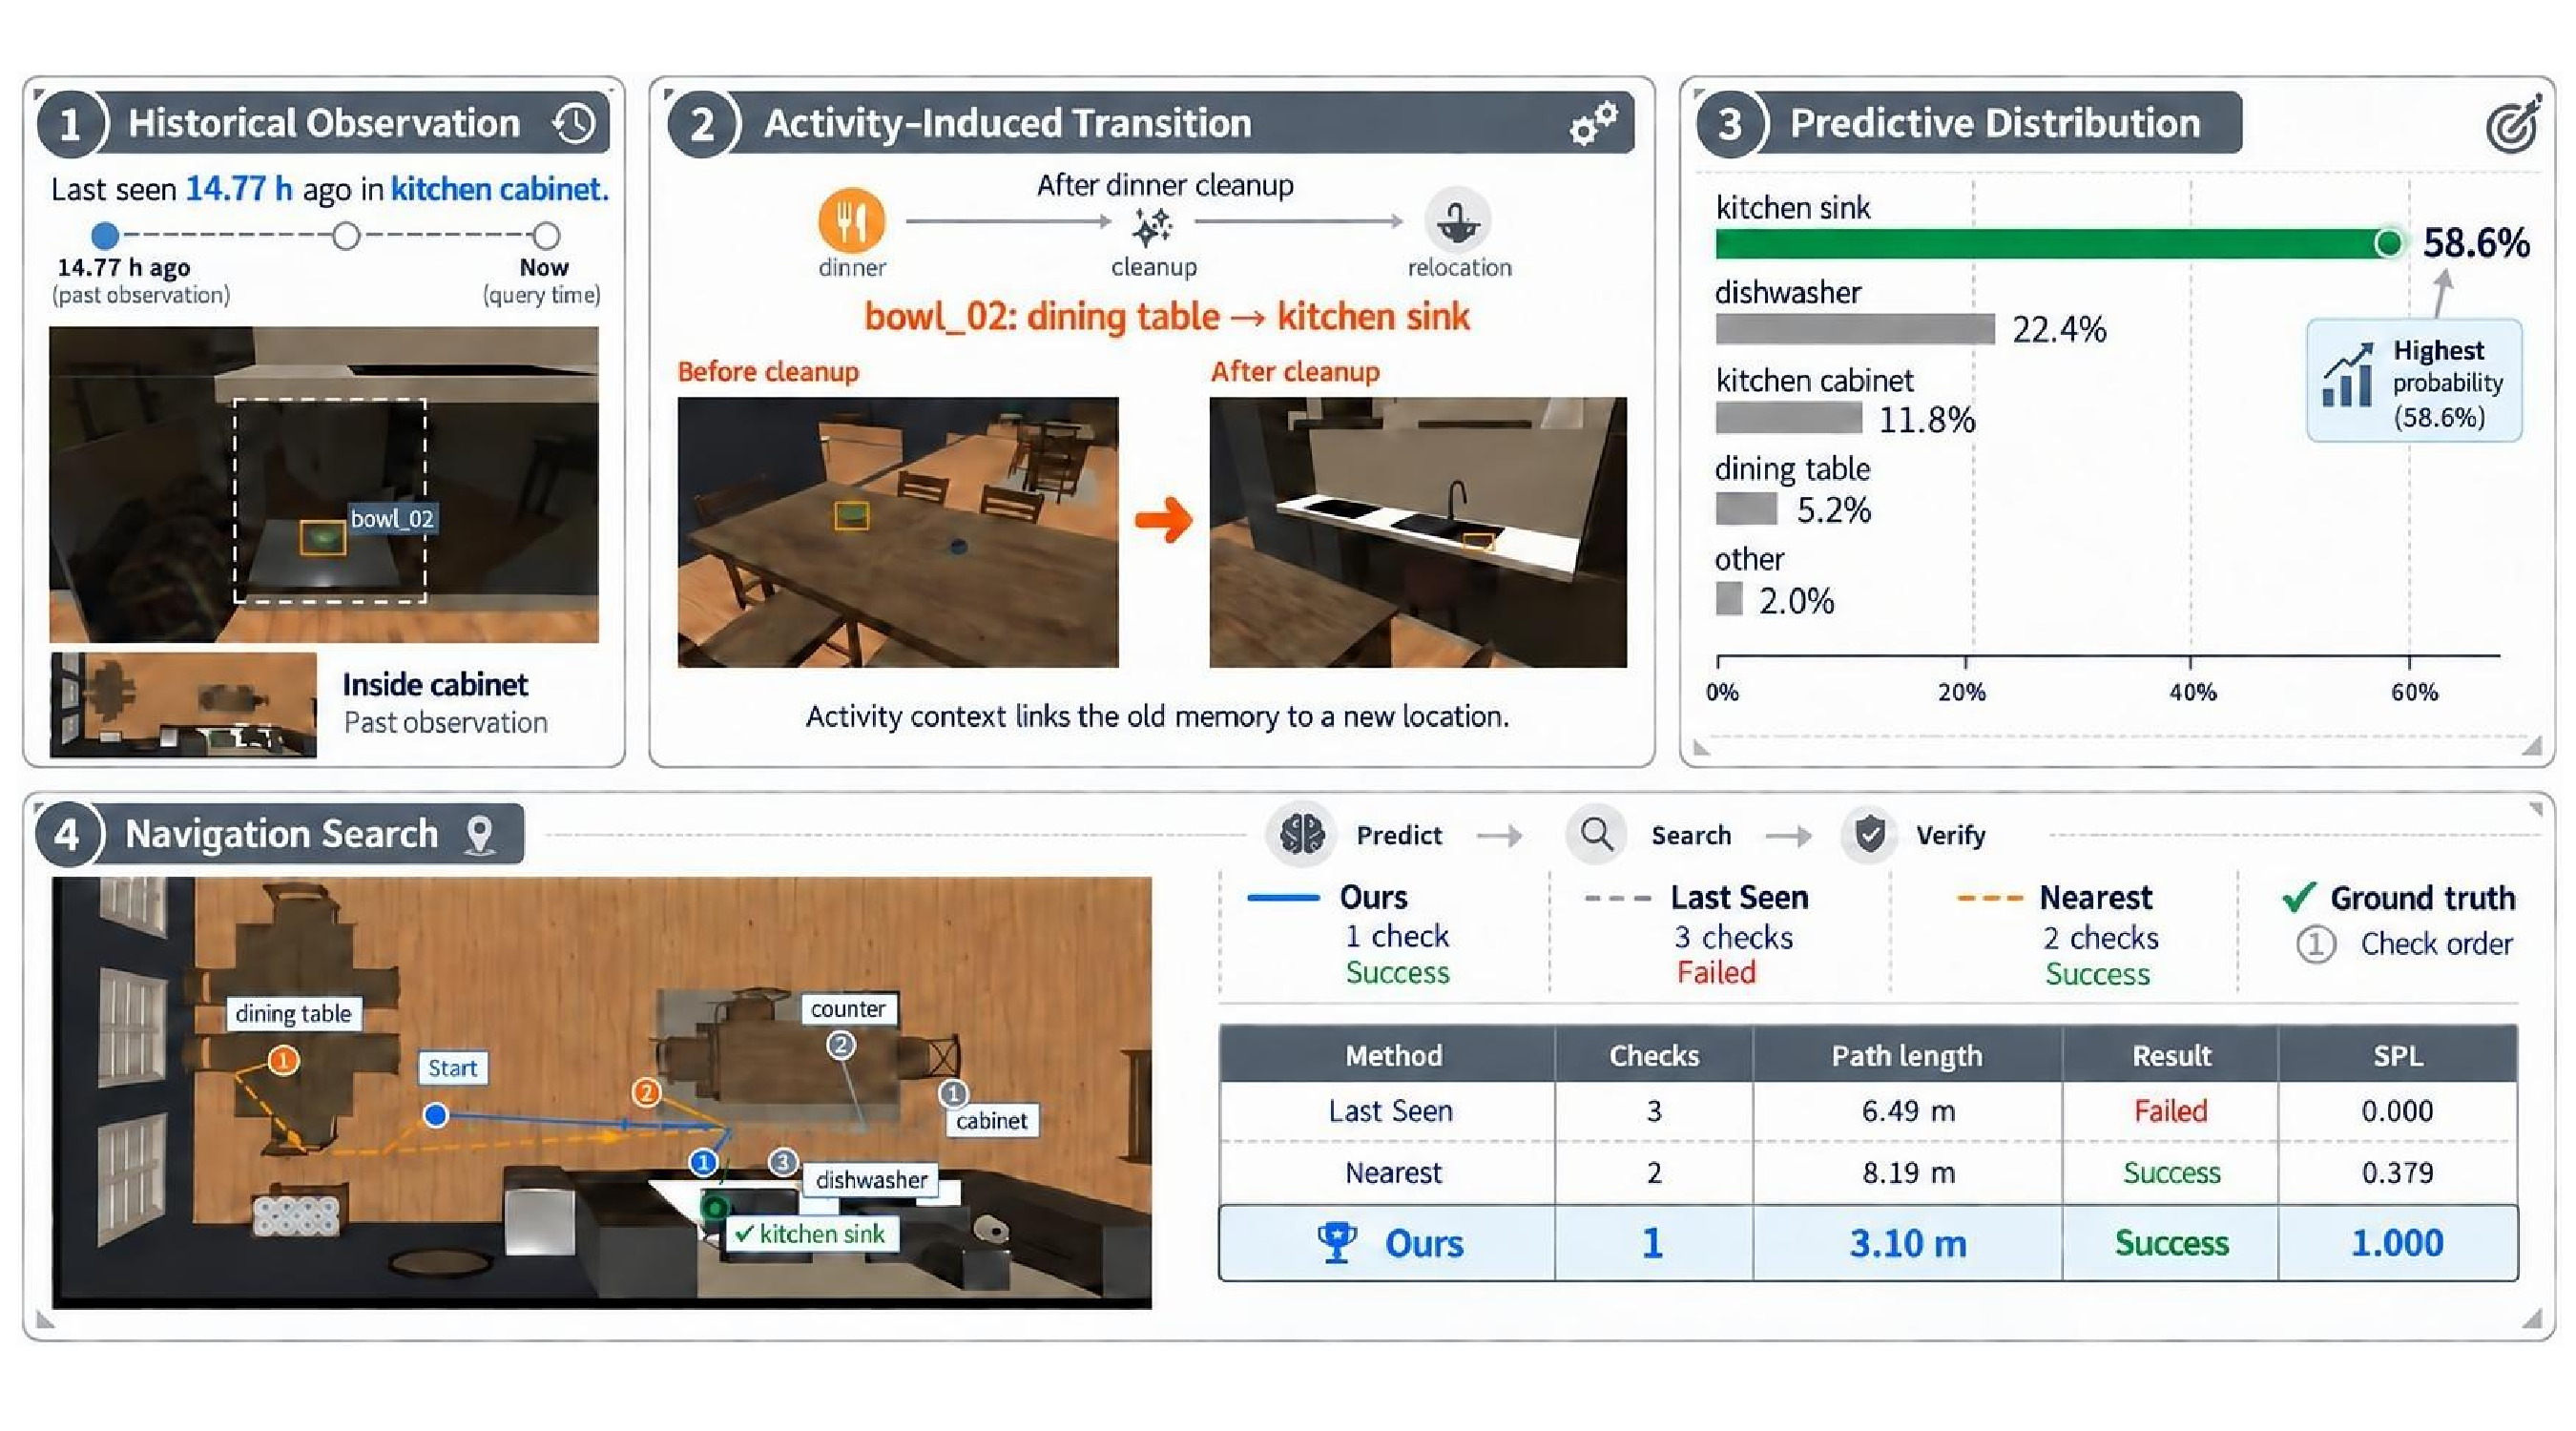
\includegraphics[width=\linewidth]{figures/P4D_CaseStudy.pdf}
    \caption{Predictive, last-seen, and nearest-first search on \evolvingworldbench{}.}
    \label{fig:p4d_case_study}
\end{figure}

\begin{table*}[!t]
\centering
\caption{Online-dynamic navigation on N4 episodes with target motion during execution.
Success rates are reported in \%; excess distance is reported in m.}
\label{tab:n4-online}
\scriptsize
\setlength{\tabcolsep}{8pt}
\begin{tabular}{lcccc}
\toprule
\textbf{Method} & \textbf{Dynamic SR $\uparrow$} &
\makecell{\textbf{Online Recovery}\\\textbf{SR $\uparrow$}} &
\makecell{\textbf{Excess Distance}\\\textbf{(m) $\downarrow$}} &
\makecell{\textbf{Revisit Success}\\\textbf{$\uparrow$}}\\
\midrule
SLaTe-PRO \citep{patel2023routine} & 34.7 & 21.5 & 18.9 & 8.7\\
SGM+NEP \citep{kurenkov2023dynamic} & 41.3 & 27.8 & 15.6 & 12.4\\
FlowMaps \citep{argenziano2026flowmaps} & 29.6 & 18.9 & 22.4 & 6.5\\
PredictiveGraphs \citep{saavedraruiz2026predictivegraphs} & 46.8 & 36.7 & 13.2 & 18.9\\
\rowcolor{tblours}\textbf{\evolvingworldnav{} (ours)} &
\textbf{65.2} & \textbf{58.7} & \textbf{8.4} & \textbf{32.6}\\
\bottomrule
\end{tabular}
\end{table*}

Relative to PredictiveGraphs, \evolvingworldnav{} improves Dynamic SR by 18.4
percentage points and Online Recovery SR by 22.0 percentage points, reduces
excess distance by 4.8\,m, and increases Revisit Success by 13.7 percentage points.
These results directly test the contribution of execution-time updates:
current-time propagation and time-valid evidence rounds allow the agent to
recover after a target moves, while candidate reopening allows productive
revisits to previously inspected locations.

\begin{wraptable}[7]{r}{0.63\linewidth}
\vspace{-0.7\baselineskip}
\caption{Primary LYNX M20 search results.}
\label{tab:real-main}
\centering
\scriptsize
\setlength{\tabcolsep}{2.2pt}
\resizebox{\linewidth}{!}{%
\begin{tabular}{@{}lrrrrrr@{}}
\toprule
Method &
\makecell{First-Inspection\\SR $\uparrow$} &
\makecell{Search\\SR $\uparrow$} &
\makecell{Recovery\\SR $\uparrow$} &
\makecell{Dist.\\(m) $\downarrow$} &
\makecell{Time\\(s) $\downarrow$} &
\makecell{Inspect.\\$\downarrow$} \\
\midrule
Last Seen + Search & 17.2 & 26.6 & 12.8 & 56.2 & 284 & 2.19 \\
Time Frequency & 21.9 & 31.3 & 14.0 & 52.9 & 277 & 2.05 \\
Retrieval + Reasoning & 26.6 & 37.5 & 17.1 & 50.3 & 281 & 2.03 \\
\rowcolor{tblours}\textbf{\evolvingworldnav{}} &
\textbf{34.4} & \textbf{48.4} & \textbf{24.3} &
\textbf{43.8} & \textbf{248} & \textbf{1.84} \\
\bottomrule
\end{tabular}%
}
\end{wraptable}

\paragraph{Generalization and physical deployment.}
Across five simulation environments, \evolvingworldnav{} achieves the highest
scores on seven of ten metrics (\cref{tab:domains}). In 64 matched M20 trials,
it improves both success and efficiency (\cref{tab:real-main}); details are in
\appref{app:real-world-eval}.

These evaluations show improvements in initial destination selection across
benchmarks, recovery under execution-time motion in N4, and path length and
inspection count in robot trials using the same belief interface. The
consistent gains across these settings argue against benchmark-specific
exploration or a stronger controller as the sole explanation.

\subsection{Ablation Studies}
\label{sec:ablations}

\paragraph{Core components.}
\begin{figure}[H]
    \centering
    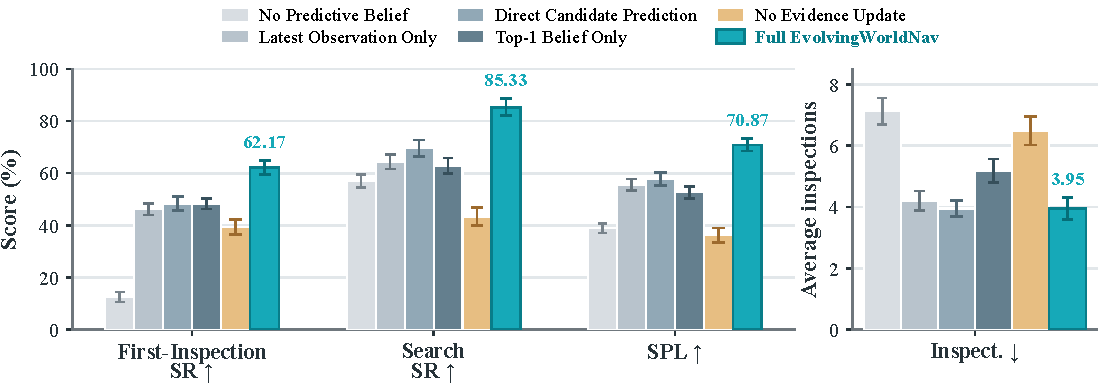
\includegraphics[width=\columnwidth]{figures/core_component_ablation_grouped.pdf}
    \caption{Core component ablation. Error bars show standard deviations over five seeds.}
    \label{fig:module_ablation}
\end{figure}

The full agent achieves 62.17\% First-Inspection SR, 85.33\% Search SR, and
70.87\% SPL with 3.95 inspections (\cref{fig:module_ablation}). Removing predictive
belief lowers First-Inspection SR to 12.51\%, while Latest Observation Only
reduces Search SR by 20.91 percentage points. Temporally persistent history
guides both initial destination selection and recovery.
Direct candidate prediction reduces First-Inspection SR and Search SR by
13.84 and 15.75 percentage points, respectively, supporting the
persistence--relocation factorization. Top-1-only search reduces Search SR by
22.41 percentage points; removing evidence updates reduces it by 42.02
percentage points and increases the inspection count to 6.48. Retaining
alternative hypotheses enables recovery, while evidence updates turn new views
into route changes; neither a better single prediction nor a larger search
budget explains these gains. No Evidence Update uses the same predictor, so its
performance gap isolates the action-time filter from offline state classification gains.


\begin{wraptable}{r}{0.64\linewidth}
\vspace{-0.7\baselineskip}
\caption{Current-state prediction on temporal and LOSO splits.}
\label{tab:predictors}
\centering
\scriptsize
\setlength{\tabcolsep}{2.3pt}
\resizebox{\linewidth}{!}{%
\begin{tabular}{lrrrrrr}
\toprule
& \multicolumn{3}{c}{Temporal} & \multicolumn{3}{c}{LOSO}\\
\cmidrule(lr){2-4}\cmidrule(lr){5-7}
Predictor & Top-1 $\uparrow$ & MRR $\uparrow$ & NLL $\downarrow$
& Top-1 $\uparrow$ & MRR $\uparrow$ & NLL $\downarrow$\\
\midrule
Last Seen & 0.00 & 0.1699 & 3.4011 & 50.00 & 0.5850 & 1.8825\\
Time Frequency & 33.85 & 0.5462 & 1.8400 & 49.53 & 0.6166 & 1.6455\\
Direct Transformer & 34.16 & 0.5586 & 1.7292 & 51.71 & 0.6884 & 1.3157\\
Shared semantic prior & 36.02 & 0.5957 & 1.5766 & 59.47 & 0.7462 & 1.0448\\
\rowcolor{tblours} & \textbf{38.24} & \textbf{0.5971} & \textbf{1.4925}
& \textbf{61.18} & \textbf{0.7523} & \textbf{0.9778}\\
\rowcolor{tblours}\multirow{-2}{*}{\textbf{Ours}}
& $\pm1.42$ & $\pm0.0291$ & $\pm0.0867$
& $\pm1.53$ & $\pm0.0176$ & $\pm0.0228$\\
\bottomrule
\end{tabular}%
}
\end{wraptable}

\paragraph{Prediction and controller robustness.}
Compared with the Direct Transformer, our predictor improves Top-1 by 4.08 and
9.47 percentage points and reduces NLL by 0.2367 and 0.3379 on the temporal and
LOSO splits, respectively. It also outperforms the shared semantic prior,
supporting temporal structure beyond location frequency. Larger LOSO gains
indicate transfer beyond scene-specific destination statistics, while lower NLL
provides more useful recovery alternatives. Additional ablations are in
\appref{app:experimental-results}.
